\documentclass[10pt]{article}
%\pagestyle{headings}

\oddsidemargin 0.0in
\evensidemargin 0.0in
\textwidth 6.0in
\topmargin 0.2in
\footskip 20pt
\textheight 8.5in

\usepackage{hyperref,color,graphicx,mathrsfs,pdflscape,datetime}
\usepackage[numbers,sort]{natbib}
\hypersetup{colorlinks,%
            citecolor=blue,%
            linkcolor=blue,%
            filecolor=blue,%
            urlcolor=red}

\bibliographystyle{unsrtnat}
\renewcommand{\rmdefault}{phv}

	\begin{document}
{\noindent\Large{\textbf{Signal/background classification in NEXT with DNNs}}}\\
Updated: \today\\ %, at \ampmtime \\

\noindent One of the most important aspects of the NEXT experiment is its ability to reconstruct the ionization tracks produced when energetic electrons deposit their
energy in the high pressure xenon gas present inside the NEXT detector.  Because many natural radioactive processes can produce energy depositions with an energy similar 
to that of neutrinoless double-beta decay,\footnote{For xenon, this energy is $Q_{\beta\beta} \approx 2.4$ MeV and common backgrounds include gamma rays produced by nuclear
decay of $^{208}$Tl and $^{214}$Bi.} and because neutrinoless double-beta decay is so rare, we will likely see many events in NEXT with energies that make them look like they could be
neutrinoless double-beta decay.  This will occur despite the shielding provided by the many meters of rock in the Pyrenees mountains, the lead castle inside which the detector is placed, and
the copper shielding inside the detector surrounding the active region!  These \textbf{background} events must be discarded (``rejected'') while the real double-beta events - the \textbf{signal} 
events - are kept.  By just looking at the energy deposited by each event, we will be able to remove many events that do not have the energy of interest, but at some point this no longer works
because all detectors have a finite energy resolution and we will have to choose a region of energies of potential interest.  Many background events will still fall into this region.\\

\noindent NEXT has further power to reject background because the ionization track of most background events (those due to gamma rays) will be produced by a single electron while the
track of a neutrinoless double beta ($0\nu\beta\beta$) event is produced by two electrons.  Because of the way energetic electrons lose energy in gaseous detectors, these two types of
ionization tracks will, most of the time, look distinctly different.  In particular, energetic electrons ionize xenon atoms at a lower density when they have higher energy, and the ionization density
increases as the electron loses energy.  Energetic electrons are also subject to less multiple scattering\footnote{Electron multiple scattering is the phenomenon responsible for
causing energetic electrons to undergo sudden sharp changes in direction while depositing their energy.} at higher energies than at lower energies.  Thus a single-electron track will look smoother
near the beginning with less energy deposited per unit distance, and more distorted near the end, with a ``blob'' of higher-density energy deposition at the end.  A track produced by two electrons
emitted from a common vertex (such as in $0\nu\beta\beta$) will be smoother and less dense near the vertex and have two such ``blobs'' at the ends.\\

\noindent The NEXT detector will reconstruct ionization tracks, providing a list of values $(x,y,z,E)$ called ``hits.''  Space is then divided up into small rectangular volumes called ``voxels,'' and
the energy from each hit is added into the voxel in which it is located.  This ``voxelized'' track is what we will work with.  In fact, we will only be working with simulated events (generated using
a Monte Carlo simulation produced by detector simulation software such as GEANT4\cite{GEANT4}) for which a single,
fully-connected voxelized track was reconstructed.  Our focus will be on training DNNs to tell the difference between a ``signal'' and ``background'' event under these simplified circumstances.  See figures \ref{fig_bgexample} and \ref{fig_siexample} for examples 
of signal and background events voxelized in volumes of 2x2x2 cubic mm.  Much detail can be seen with this relatively small
voxel size (impractical with the current NEXT technology and at the lower limit of what seems to be obtainable even with future
advances).  We currently expect to use 10x10x5 mm$^3$ voxels in NEXT, and for these exercises we will begin working with
10x10x10 mm$^3$, mostly because it means a smaller event size and is therefore less computationally expensive.

\begin{figure}[!ht]
	\centering
	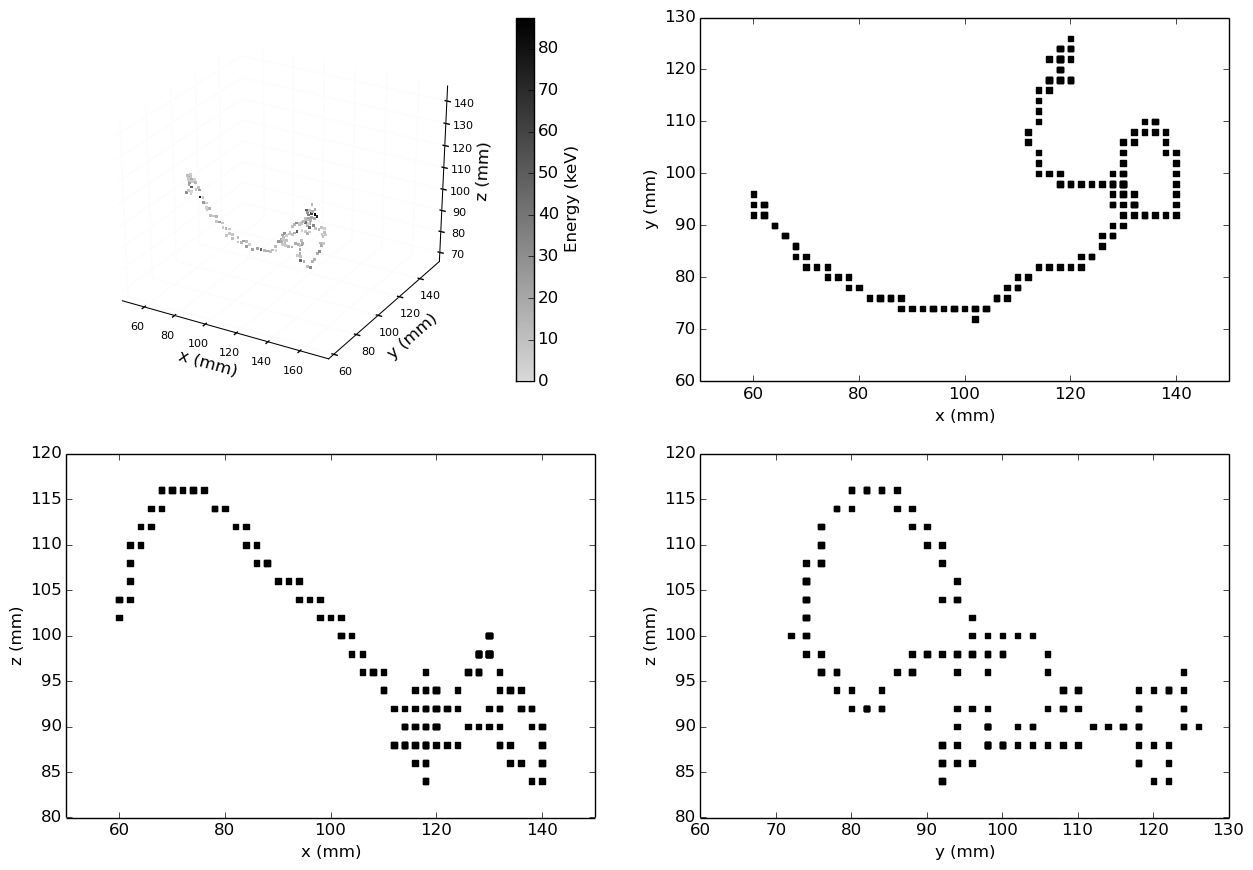
\includegraphics[scale=0.4]{fig/plt_dnn3d_NEXT100_Paolina222_v2x2x2_r200x200x200_bg_5.png}
	\caption{\label{fig_bgexample}Example of a simulated \textbf{background} event voxelized in volumes of 2x2x2 mm$^3$.}
\end{figure}

\begin{figure}[!ht]
	\centering
	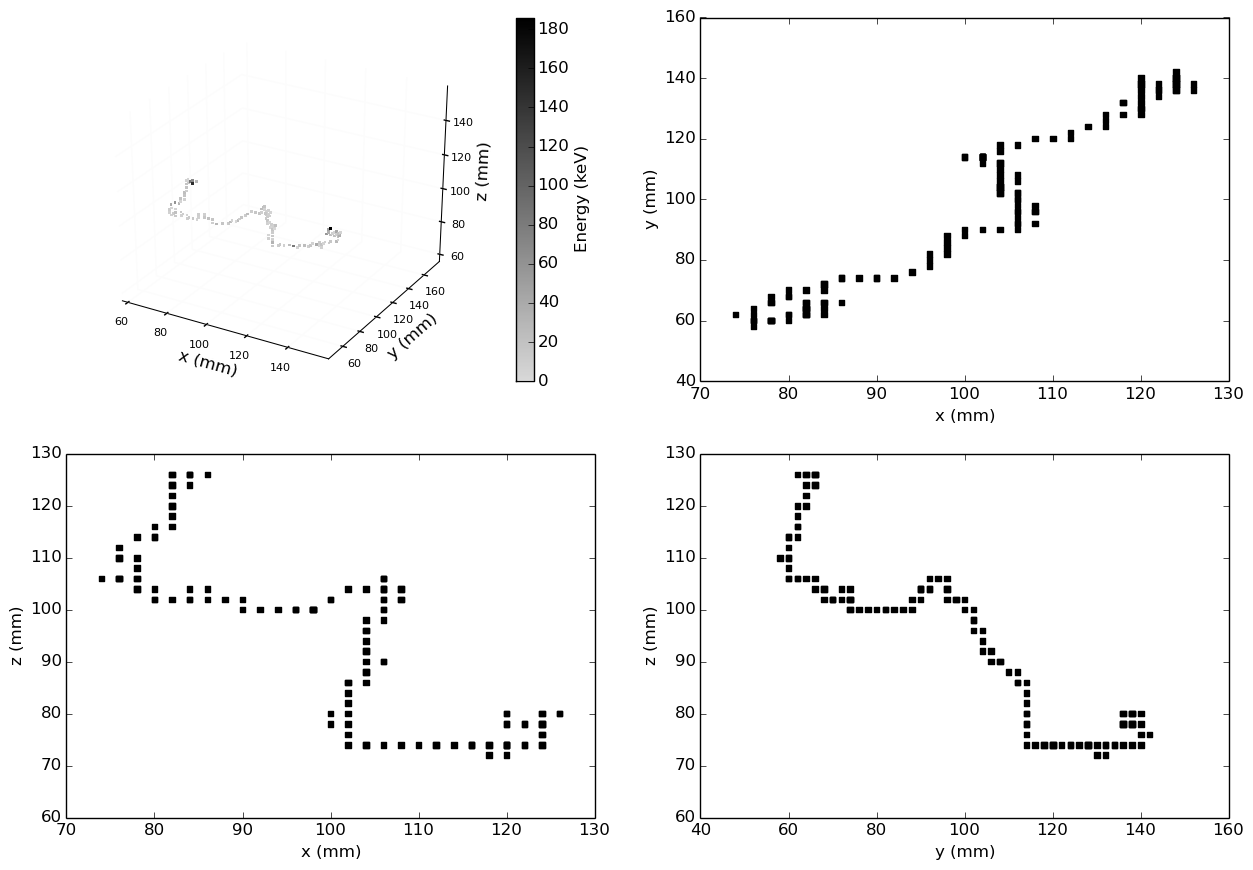
\includegraphics[scale=0.4]{fig/plt_dnn3d_NEXT100_Paolina222_v2x2x2_r200x200x200_si_2.png}
	\caption{\label{fig_siexample}Example of a simulated \textbf{signal} event voxelized in volumes of 2x2x2 mm$^3$.}
\end{figure}

\section{Running a basic neural network analysis}\label{s_basicanalysis}
\noindent First we will focus on the logistics necessary to run a simple neural network analysis, including the choice of code and data formats 
and the necessary computer commands.

\subsection{Overview of computing tools used}\label{ss_computingtools}
\noindent The following is a brief summary of the key tools used in this analysis:

\begin{enumerate}
	\item[\textbullet] \textbf{Python}: most of the code we will run is written in Python.  With previous programming knowledge, 
	Python should be readable, and a quick search on the Internet will probably provide code for how to perform specific operations
	(such as reading/writing to a file, creating a multidimensional array ...) when in doubt.  It is a good idea to obtain some
	familiarity with the basics of the language, and for this, working through sections 1-4 of 
	\href{https://docs.python.org/2/tutorial/}{this Python tutorial} (or a similar one) would be helpful.  Several widely-used
	Python libraries will be used including \href{http://matplotlib.org}{matplotlib}, \href{http://www.numpy.org}{numpy}, and \href{http://www.h5py.org}{h5py}.
	\item[\textbullet] \textbf{Linux}: the analysis will be done in a Linux environment.  In most cases the necessary commands
	will be mentioned in this document and some miscellaneous commands can be found in appendix \ref{s_app_linux}.  As
	the code and files that will be edited are stored on another machine accessed remotely, it will be helpful to become familiar
	with a text editor such as \href{https://www.gnu.org/software/emacs}{emacs}.
	\item[\textbullet] \textbf{\href{https://www.tensorflow.org}{TensorFlow}}: this is a Python library that facilitates the creation and 
	training of neural networks.  Another library based on C$++$ which we will not use, at least initially, is \href{http://caffe.berkeleyvision.org}{Caffe}.
	\item[\textbullet] \textbf{\href{https://git-scm.com}{git}}: a version control system that allows you to store, update, and share
	code with multiple people at the same time.  It is used when multiple people are working on the same project.  The basics of Git can be learned quickly from \href{https://try.github.io}{this online tutorial}.
\end{enumerate}

\noindent At this point it would be helpful to spend several minutes glancing through the links in the above list, then
move on to section \ref{ss_basicanalysis}, which is a walk-through of an initial run of the code and
an introduction to the main ideas.

\subsection{Running the neural net analysis}\label{ss_basicanalysis}
\noindent Here we will run an analysis on simulated NEXT-100 data using a basic neural network (in this example, it is in fact not a \emph{deep} neural network, just a neural network with
a single hidden layer).  We start by first 
logging in remotely to the machine \verb|analysis01|.  Open a terminal and enter

\begin{verbatim}
 ssh -X name@analysis01.ific.uv.es
\end{verbatim}

\noindent where \verb|name| is to be replaced by your user name.  Type the password and hit enter.  You're now 
logged into the machine and can start.  First we will create a main directory for our dnn work.  Enter

\begin{verbatim}
 mkdir dnn
\end{verbatim}

\noindent We can now see this directory and any others that are there by entering the command \verb|ls|.  Now move into the newly
created directory by typing

\begin{verbatim}
 cd dnn
\end{verbatim}

\noindent We can obtain the relevant code by typing

\begin{verbatim}
 git clone https://github.com/jerenner/dnntools.git
\end{verbatim}

\noindent This will download the relevant code and place it in a subfolder called \verb|dnntools|.  We will now set up the code
to be run.  Move to this new directory (\verb|cd dnntools|), and there should be several Python scripts:

\begin{enumerate}
	\item[--] \verb|dnninputs.py|: used to define input parameters
	\item[--] \verb|dnntrain.py|: used to run the training based on the specified parameters
	\item[--] \verb|dnnplot.py|: used to make key plots of the data and results
\end{enumerate}

\noindent Now open the file \verb|dnninputs.py|

\begin{verbatim}
 emacs dnninputs.py
\end{verbatim}

\noindent and set the inputs.

\begin{quotation}
	$\rightarrow$ \textbf{\emph{Note:}} running a Unix command followed by the amperstand \verb|&| will run that command in a separate Unix shell so you can continue issuing further commands without having to wait until it finishes.  For example: \verb|emacs dnninputs.py &|
\end{quotation}

\noindent Each input is explained in the comments in the file.  Set the data file to the name of the \verb|.h5| file (without the \verb|.h5|) corresponding to NEXT-100 simulated events with 10x10x10 mm$^3$ voxels.  The correct name would be  \verb|vox_dnn3d_NEXT100_Paolina222_v10x10x10_r200x200x200| (this file should be installed in the subfolder \verb|data|
of your home directory - type \verb|cd| and hit enter to navigate there directly).

\begin{quotation}
	$\rightarrow$ \textbf{\emph{Note:}} the Unix command \verb|pwd| will show you what directory you are currently in.
\end{quotation}

\noindent The variable \verb|rdir| holds the name of the directory to which the output information from different analyses will be
written.  For now this can be set to a directory called \verb|run| also in your home directory (so, \verb|/home/user/run|, replacing \verb|user| by your username).  The run name can be chosen arbitrarily.\\

%\begin{quotation}
%	$\rightarrow$ \textbf{\emph{Note:}} running this code requires several Python packages (TensorFlow, h5py, and others) which have already been pre-installed.  It also requires, for possible later use, the code from \href{https://github.com/ethereon/caffe-tensorflow}{caffe-tensorflow}, which can be used to convert neural networks used in the Caffe code to TensorFlow neural networks, and should also be pre-installed.
%\end{quotation}

\noindent Once all parameters in \verb|dnninputs.py| have been set (for a first run, all parameters except \verb|datdir| and
\verb|rdir| which require correct folder names, can be left
unchanged), save the file.  Now the training step can be run:

\begin{verbatim}
 python dnntrain.py &
\end{verbatim}

\noindent This step will take some time to run (about 16 minutes for 30 epochs of 10000 training events).  Progress can be checked by looking at the .log file in the ``run directory,'' that is, the 
subdirectory named with the value set to the variable \verb|rname| in \verb|dnninputs.py|, in the directory set as the variable 
\verb|rdir| in \verb|dnninputs.py|.  Also, a list of running processes in the current
login session can be viewed with the linux command \verb|ps|.  Note that if you have logged out of the machine and then logged
back in, a list of all processes running for a given user can be produced with the command

\begin{verbatim}
 ps aux | grep username
\end{verbatim}

\noindent where \verb|username| is replaced by your Linux user name.  Once the process is finished, one can plot the classification
accuracy of the training and validation data throughout the training process by using the \verb|dnnplot.py| script

\begin{verbatim}
 python dnnplot.py summary
\end{verbatim}

\noindent The plot should have appeared in the \verb|plt| subdirectory of the ``run directory.''  It can be opened using 

\begin{verbatim}
 gnome-open run_name_summary.png
\end{verbatim}

\noindent where \verb|run_name| will be \verb|rname| from \verb|dnninputs.py|.  This file can be transferred to the local machine
with \verb|scp| (see section \ref{ss_app_sshscp}).  It should look something like figure \ref{fig_basicsummary}.\\

\begin{figure}[!ht]
	\centering
	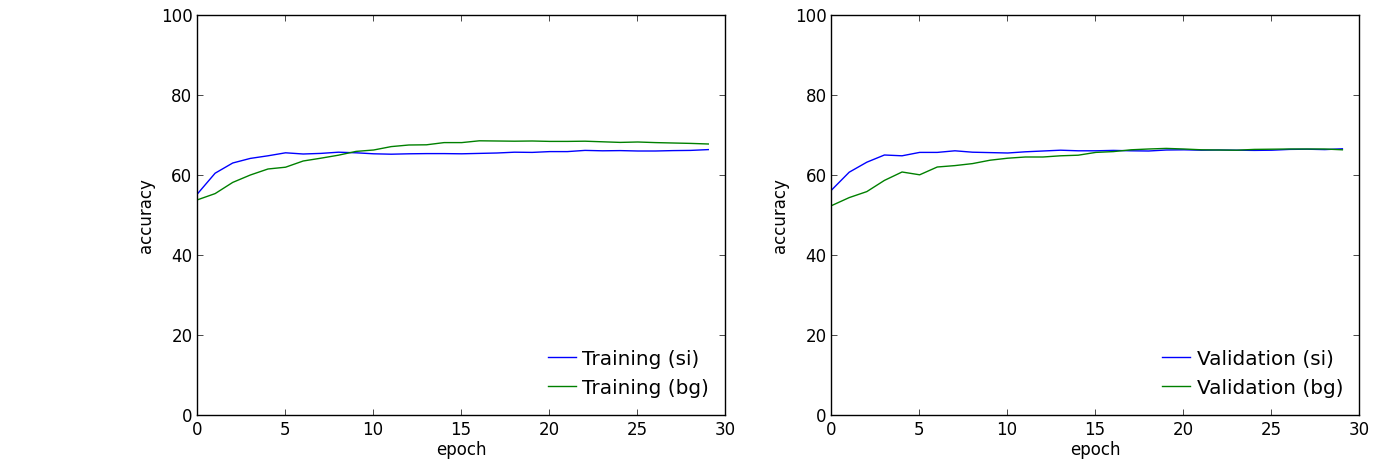
\includegraphics[scale=0.425]{fig/dnn3d_NEXT100_Paolina222_v10x10x10_r200x200x200_basic_summary.png}
	\caption{\label{fig_basicsummary}Summary plot for basic neural net classification of NEXT-100 simulated signal and background events (10x10x10 mm$^3$ voxels).}
\end{figure}

\noindent Note that the validation accuracy converges to about 67\% (the file with name beginning with ``accuracy'' in the \verb|acc| subdirectory of the run directory can be checked for the 
numerical values on the plots - the 2nd and 3rd columns are the training signal and background accuracies respectively, and the 6th and 7th columns are the validation signal and background
accuracies respectively).  This is not so good - for both signal and background, the neural net is classifying only 17\% better than a random guess.  This can be improved, and in the next
section we will see how.  At this point, it would be helpful to

\begin{enumerate}
	\item[-] review the directories and files created/edited/run in this section to get a clear idea of where everything is at.
	\item[-] work through key parts (sections 1-4) of the \href{https://docs.python.org/2/tutorial/}{Python tutorial} discussed in section \ref{ss_computingtools}, if this has not already been done.
	\item[-] read the \href{https://www.tensorflow.org/versions/r0.7/tutorials/mnist/beginners/index.html}{basic MNIST tutorial} for TensorFlow.  Compare the code introduced throughout the tutorial
	to the code in the \verb|MNISTbasic_net| function of \verb|dnntools/nets/neuralnets.py|.  The code defining the layout of the neural network described in this tutorial was placed in the 
	\verb|MNISTbasic_net| function to describe the neural net
	in the analysis we just ran.  We were not solving the same problem as in the tutorial (handwriting recognition) but using the same neural net to solve our problem of track classification.  In the next section, we will set up a 
	more advanced neural network in a similar way.
\end{enumerate}

\section{Implementing an improved DNN}\label{s_mnistadv}
\noindent Next we will modify the analysis to use the DNN from the \href{https://www.tensorflow.org/versions/r0.7/tutorials/mnist/pros/index.html}{advanced MNIST tutorial}.  First read through this tutorial, noting again that
we will not be solving the same problem but just using the DNN described.  The idea now is to set up the same neural net within the dnntools code.  First we will discuss some more details
about how the neural net is set up.

\subsection{Neural net setup}
\noindent The neural net is set up in the \verb|net_setup| function of \verb|dnntrain.py|.  The details of the specific neural net that is used in the analysis are described in \verb|neuralnets.py|.
The specific net is chosen via the input parameter \verb|net_name| set in \verb|dnninputs.py|.  During the setup of the neural net, the 
\verb|getNet| function in \verb|neuralnets.py| is called with the specified net name, and it calls the function which defines the details of the neural net.  This function takes as an argument
the TensorFlow placeholder object \verb|x_input| described below (section \ref{ss_nninput}).

\subsection{The neural net input layer}\label{ss_nninput}
\noindent For this analysis and that of the previous section, the input layer to the neural net is an array of \verb|3*npix| values, where \verb|npix| is the number of pixels in a 2D 
projection of a single 3D event.  If we are working with voxels of size 10 mm in a 200x200x200 mm$^3$ volume, a 2D projection would be 200x200 mm$^2$ or $20 \times 20 = 400$
pixels.  We are using 3 different projections (xy, yz, and xz) which can be thought of as corresponding to three different ``color channels'' in an image (R, G, B), and therefore need 
\verb|3*npix| values in our input array instead of \verb|npix| values.  A TensorFlow ``placeholder'' is created:

\begin{verbatim}
 x_input = tf.placeholder(tf.float32, [batch_size, 3*npix])
\end{verbatim}

\noindent which sets up a matrix of \verb|batch_size| arrays that will contain the 3 projections for each event.  We present TensorFlow with batches of training events rather than feeding it events one by one - this is why the input placeholder has an additional dimension of \verb|batch_size|.  Note that, as in the TensorFlow tutorials, we could have placed \verb|None| as this dimension and 
TensorFlow will adjust the size automatically according to the size of the batch of events we eventually use to do the training.  We are specifying the batch size explicitly because it avoids problems 
when trying to train models converted from Caffe, which we may eventually want to do.

\subsection{Preparing the function}
\noindent In this section, the goal is to write a function \verb|MNISTadv_net| that describes the ``Multilayer Convolutional Network'' 
discussed in the advanced MNIST tutorial.  This means changing \verb|net_name| in \verb|dnninputs.py| to a string describing the net, perhaps \verb|"MNISTadv"|, and then updating the \verb|getNet| function to call the new function when this name is passed:

\begin{verbatim}
 if(name == "MNISTadv"):
     return MNISTadv_net(x_input)
\end{verbatim}

\noindent \textbf{Now use the code in the TensorFlow tutorial to define the first convolutional layer, second convolutional layer, densely connected layer, dropout layer, and readout layer.}  Below is some additional information that will help with this.\\

\noindent The readout 
(output) layer in the case of both MNIST neural nets is a \verb|softmax| layer.  This is what needs to be returned by the function so that it can be used in \verb|dnntrain.py|.  Note we need to
make several changes to the TensorFlow code to fit our particular application.  First, our \verb|3*npix| input actually contains \verb|npix| groups of 3 values (r, g, and b for xy, yz, and xz projections) corresponding 
to the energy values in each pixel of the 2D projection:

\begin{verbatim}
 [r0, g0, b0, r1, g1, b1, r2, g2, b2, ...]
\end{verbatim}

\noindent and this needs to be resized slightly differently than in the TensorFlow tutorial:

\begin{verbatim}
 x_image = tf.reshape(x_input, [-1,pdim,pdim,3])
\end{verbatim}

\noindent Note here we the last number in the square brackets is 3, for the three projections and \verb|pdim| is a number calculated in \verb|dnninputs.py| that is equal to the number of
pixels per dimension for our data.  Furthermore, in creating the densely connected layer, the TensorFlow tutorial assumes 
28x28 images, so that after 2 max pooling layers (each of which reduces each dimension
by a factor of 2), we have a 7x7 image ($(28 / 2) / 2 = 7$).  In our case we need to replace those 7's by \verb|pdim / 4| (for dimension 20, this would be 5).  Overall our function would
look something like:
\newpage
\begin{verbatim}
 def MNISTadv_net(x_input):

     # Resize the array to pdim x pdim x 3
     x_image = tf.reshape(x_input, [-1,pdim,pdim,3])
     
     # ... code defining layers from TensorFlow tutorial; 
     #     the softmax layer is stored in y_conv
     
     return y_conv
\end{verbatim}

\subsection{Analysis with the advanced MNIST net}
\noindent Now the analysis can be run again as in section \ref{ss_basicanalysis}.  The run name should be changed in \verb|dnninputs.py| before this is done to avoid conflicting with the
previous run.  The run should take about 30 minutes to complete.  The corresponding summary plot should look like that shown in figure \ref{fig_advsummary}, where the validation accuracy has 
improved to about 84\% for signal and 80\% for background after 30 epochs.  Note that we may have wanted to run longer since the individual signal and background accuracies do not seem to 
have converged after 30 epochs.

\begin{figure}[!ht]
	\centering
	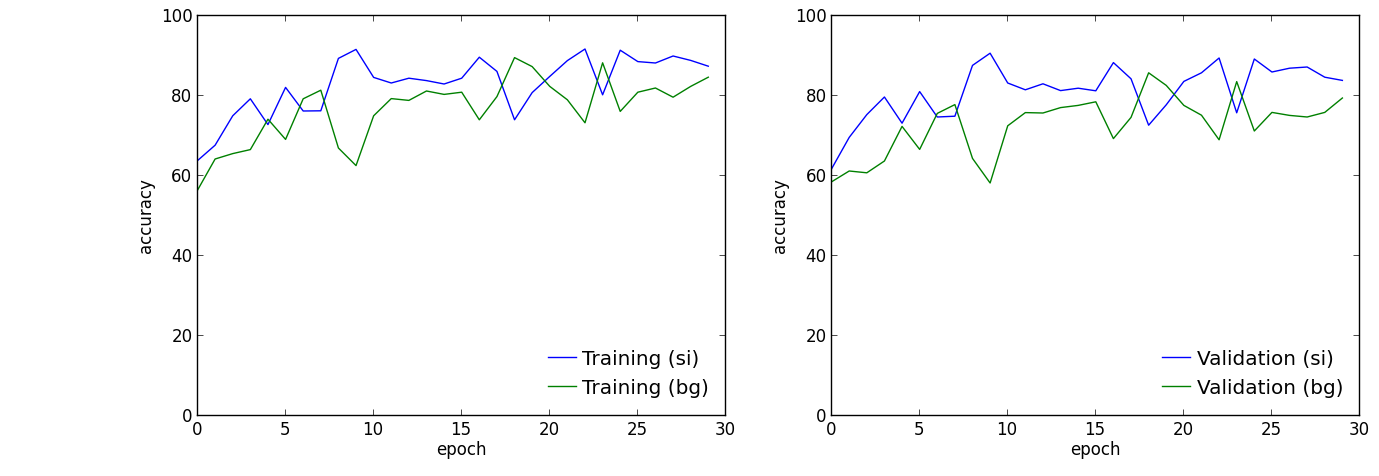
\includegraphics[scale=0.425]{fig/dnn3d_NEXT100_Paolina222_v10x10x10_r200x200x200_adv_summary.png}
	\caption{\label{fig_advsummary}Summary plot for advanced neural net classification of NEXT-100 simulated signal and background events (10x10x10 mm$^3$ voxels).}
\end{figure}

\section{Neural net optimization}
\noindent In section \ref{s_basicanalysis} we ran a basic neural net analysis, and in section \ref{s_mnistadv} we changed the design of the neural net to improve upon this analysis.
Now the question is, can we do any better?  The idea now is to use the tools we have developed and the commands available in TensorFlow to create and test better neural nets.
In this case, improvements can mean either faster running time or, more importantly, better accuracy.

\appendix
\section{Deep neural networks}\label{s_app_dnns}
\noindent Deep neural networks (DNNs) can be used to solve a variety of problems that would otherwise be extremely difficult to approach with other methods based on 
direct computation.  A clear discussion of DNNs can be found in 
\href{http://neuralnetworksanddeeplearning.com/index.html}{this book}.  

\section{HDF5 data format}\label{s_app_hdf5}
\noindent The data used in these exercises is stored in the \href{https://www.hdfgroup.org/HDF5}{HDF5 format} and can be read 
using the Python package \href{http://www.h5py.org}{h5py}.  The data are a list of voxel coordinates, \emph{in pixels, not mm} and 
a corresponding energy.  Because the voxel coordinates are in pixels, they must be multiplied by the voxel size in mm to get
the actual coordinate in mm.  Therefore for 10x10x10 mm$^3$ voxels, the voxel at $(1,2,1)$ has y-coordinate 
$2\times 10 = 20$ mm.  The energies are stored in keV.  All information is stored in HDF5 objects, one per event, named \verb|trkX|, where \verb|X| is a number
corresponding to the event number.  For example, to open a data file named \verb|vox_dnn3d_NEXT100_Paolina222_v10x10x10_r200x200x200_bg| and access the
stored lists of x, y, and z voxel coordinates, and the stored list of energies:

\begin{verbatim}
h5f = h5py.File("vox_dnn3d_NEXT100_Paolina222_v10x10x10_r200x200x200_bg.h5", 'r')
trkobj = h5f['trk100']
trk_vox_x = trkobj[0]
trk_vox_y = trkobj[1]
trk_vox_z = trkobj[2]
trk_vox_E = trkobj[3]
\end{verbatim}

\noindent Note again that the voxels span a volume of 200x200x200 mm and have 10 mm dimensions meaning that the coordinates will run from 0 to 19 in each dimension.  Also,
a voxel is only stored if it has nonzero energy.

\section{Linux environment}\label{s_app_linux}
\noindent Mac OS supports Unix commands - just open the application ``Terminal'' and you can start issuing such commands.  A useful more powerful terminal for Mac OS is iTerm2
(\href{https://www.iterm2.com}{https://www.iterm2.com}).

\subsection{ssh and scp}\label{ss_app_sshscp}
\noindent Two useful commands that can be used to communicate with other Linux/Unix machines are \verb|ssh| and \verb|scp|.  To connect to another machine using \verb|ssh|, use

\begin{verbatim}
 ssh -X user@machine.address
\end{verbatim}

\noindent where \verb|user| is the user name and \verb|machine.address| is the name and address of the machine to which to connect (for example, \verb|analysis01.ific.uv.es|).  Note that creating a new text
file (named, for example \verb|analysis01|) and placing in it the above command, then issuing the command,

\begin{verbatim}
 chmod a+x analysis01
\end{verbatim}

\noindent the file becomes ``executable'' so that as a shortcut one can execute the ssh command just by running \verb|./analysis01|.\\

\noindent The \verb|scp| command allows one to transfer files to or from the specified machine.  For example, to transfer file \verb|datfile.txt| in the current directory of the current machine to the directory 
\verb|/home/user/data| on machine \verb|analysis01.ific.uv.es| via login \verb|user|,

\begin{verbatim}
 scp datfile.txt user@analysis01.ific.uv.es:/home/user/data
\end{verbatim}

\subsection{Some Unix commands}\label{ss_app_commands}
\noindent Here are some basic Unix commands.

\subsubsection{\texttt{cat}}
\noindent This command can be used to print the contents of a file to the terminal.  Example: 

\begin{verbatim}
  cat code.py
\end{verbatim}

\subsubsection{\texttt{cd}}
\noindent This command changes directories.  For example, if one wanted to change to the directory ``folder'' contained in the current directory one could type:

\begin{verbatim}
  cd folder
\end{verbatim}

\noindent Just typing \verb|cd| will take you straight to your ``home'' directory no matter what directory you are currently in.\\

\noindent The ``parent'' directory (the one containing the current directory) is represented by two dots \texttt{..} in Unix/Cygwin commands.  The following command will change directories to the parent directory.
\begin{verbatim}
  cd ..
\end{verbatim}
  
\subsubsection{\texttt{cp <file> <destination>}}
\noindent This command copies a file to the location specified (similar to \texttt{mv}, except the original file is kept).  To make a copy of ``data.c'' located in the directory src and name it ``old\_data.c'':

\begin{verbatim}
  cp data.h5 old_data.h5
\end{verbatim}

\subsubsection{\texttt{exit}}
\noindent This command is used to quit the current Linux terminal.

%\subsubsection{\texttt{gcc <source\_file.c> -o <out\_file>}}
%\noindent This command is used to compile a C program.  For example, to compile the file \texttt{source.c} into the program called \texttt{pgm}:
%
%\begin{verbatim}
%  gcc source.c -o pgm
%\end{verbatim}
      
\subsubsection{\texttt{ls}}
\noindent This command lists all the files in the current directory.

\subsubsection{\texttt{mkdir} \textless dir\textgreater}
\noindent This command creates a new directory specified by \textless dir\textgreater.  To create a directory called \texttt{folder} in the current directory:

\begin{verbatim}
  mkdir folder
\end{verbatim}
	  
\subsubsection{\texttt{mv <file> <destination>}}
\noindent This command moves a file to the specified location.  For example to move the file ``code.py'' into a directory called ``srcdir'' that is contained in the current directory:

\begin{verbatim}
  mv code.py srcdir
\end{verbatim}

\noindent You can also use \texttt{mv} to rename files.  To rename ``code.py''' to ``old\_code.py'':
\begin{verbatim}
  mv code.py old_code.py
\end{verbatim}

\noindent Note that you can also move and rename at the same time.  The following renames ``code.py'' to ``old\_code.py'' and moves it to directory called ``srcdir'':
\begin{verbatim}
  mv code.py srcdir/old_code.py
\end{verbatim}

\noindent Note that in \texttt{mv} and \texttt{cp} and other commands, the current directory is specified by (\texttt{.}) - a single dot.  To move ``code.py'' from the directory ``srcdir'' to the current directory:
\begin{verbatim}
  mv srcdir/code.py .
\end{verbatim}  

\bibliography{dnnopt_doc}
\end{document}